This chapter provides a detailed architectural design of Students\&Companies, starting with a high-level overview of the system's design choices and their rationale.
It then explores the component view, illustrating major system modules and their interactions using various UML diagrams.
A deployment view follows, showing how software components distribute across hardware nodes.
Runtime views are then presented through sequence diagrams depicting key system operations.
The chapter concludes with a discussion of chosen architectural styles, patterns and other significant design decisions.

\section{Overview}
Students\&Companies requires an architecture that can efficiently handle the complex interactions between students, companies and universities while ensuring system scalability and data security.
The platform adopts a three-tier client-server architecture, separating presentation, application logic and data management into distinct layers.
This section provides an overview of the application of this architecture to the problem at hand, while a more general discussion of patterns and styles belongs in later sections.

\subsubsection{Client Tier}
At the client tier, the web app serves as the user interface, allowing students, companies and universities to access S\&C through their browsers.
The app is designed to be responsive, ensuring accessibility across various devices while maintaining a consistent user experience.

\subsubsection{Middle Tier}
The middle tier consists of three server components.

The web server handles incoming client requests, managing user sessions and providing load balancing capabilities to distribute traffic effectively across multiple instances of the application server.
The AS contains the core business logic, processing user requests to coordinating the entire internship lifecycle from application to completion.

The mail server manages the email workflow, determining when to send notifications for registration confirmations, new matches, selection updates or internship comments.
For actual email delivery, the MS integrates with an external email provider that handles the delivery infrastructure, ensuring reliable communication reaches users' inboxes.

\subsubsection{Data Tier}
The data tier employs a DBMS server to store and manage all system data.
This includes user profiles, internship positions, ongoing matches, selection processes and internship records.
The DS provides structured data storage with built-in mechanisms for maintaining data integrity through transaction management and constraint enforcement, optimizing query performance through indexing and caching, and implementing access controls and encryption for sensitive user data.

Overall, this architecture enables efficient data flow while maintaining scalability and security.
When a user interacts with the WA, their request flows through the WS to one of the AS instances, which processes it using data from the DS and triggers notifications through the MS when necessary.

\begin{figure}[h]
    \centering
    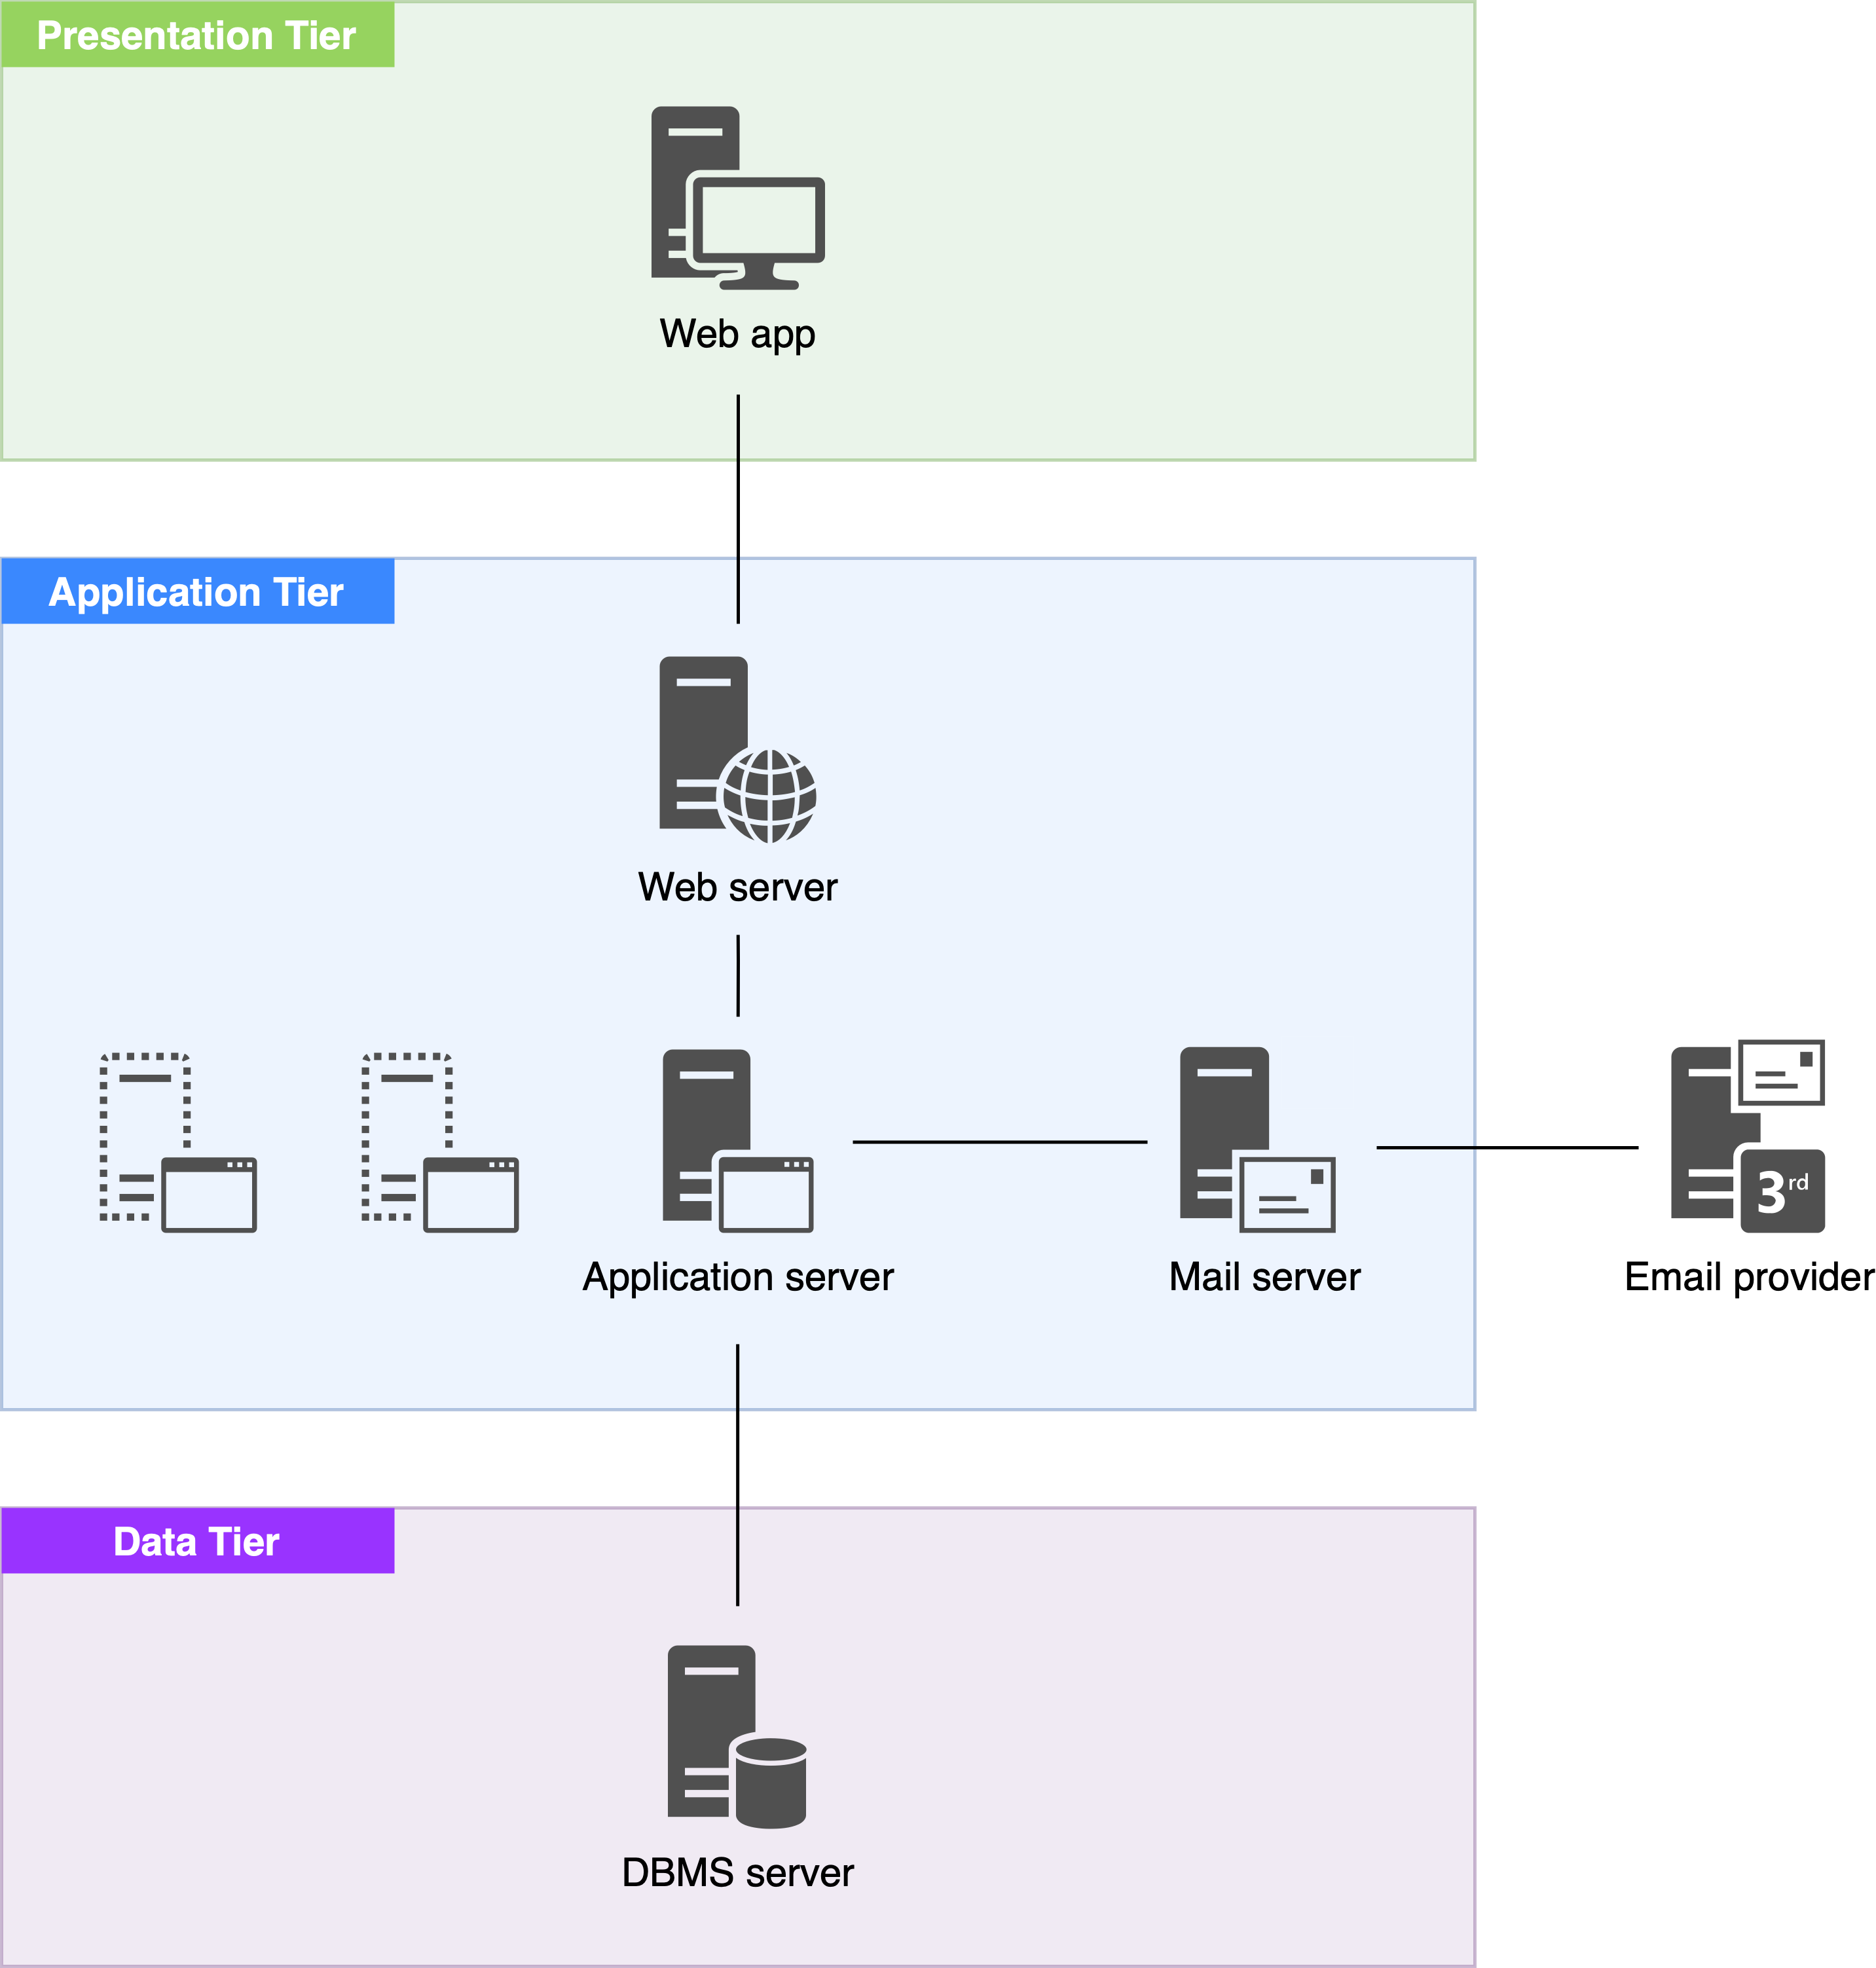
\includegraphics[width=14cm]{images/architecture.png}
    \caption{Architecture overview}
\end{figure}

\section{Component View}
\subsection{High Level Diagram}
\subsection{Low Level Diagram}
\subsection{Managers}
\section{Deployment View}
\section{Runtime View}
\section{Component Interfaces}
\section{Architectural Styles and Patterns}
\section{Other Design Decisions}
